\documentclass[pdftex]{beamer} 
\usepackage{graphicx}
\usepackage{amsmath,amssymb,amsthm} 
\usepackage{pb-diagram}
\usepackage{ucs}
\usepackage[utf8x]{inputenc}
\usepackage[russian]{babel}
\usepackage{epstopdf}
\usepackage{multicol}
\usepackage{cancel}

\usepackage{amsfonts}

%%%%%%%%%%%%%%%%%%%%%%%%%%%%%%%%%%%%%%%%%%%%%%%%%%%%%%%%%%%%%%%%%%%%%%%%%%%%%%%%%%%%%%%%%%%%%%%%%%%

%\newtheorem{theorem}{Theorem}
%% \newtheorem{acknowledgement}[theorem]{Acknowledgement}
%% \newtheorem{algorithm}[theorem]{Algorithm}
%% \newtheorem{axiom}[theorem]{Axiom}
%% \newtheorem{case}[theorem]{Case}
%% \newtheorem{claim}[theorem]{Claim}
%% \newtheorem{conclusion}[theorem]{Conclusion}
%% \newtheorem{condition}[theorem]{Condition}
%% \newtheorem{conjecture}[theorem]{Conjecture}
%% \newtheorem{mycorollary}[theorem]{Corollary}
%% \newtheorem{mycriterion}[theorem]{Criterion}
%% \newtheorem{mydefinition}[theorem]{Definition}
%% \newtheorem{myexample}[theorem]{Example}
%% \newtheorem{myexercise}[theorem]{Exercise}
%% \newtheorem{mylemma}[theorem]{Lemma}
%% \newtheorem{mynotation}[theorem]{Notation}
%% \newtheorem{myproblem}[theorem]{Problem}
%% \newtheorem{myproposition}[theorem]{Proposition}
%% \newtheorem{myremark}[theorem]{Remark}
%% \newtheorem{mysolution}[theorem]{Solution}
%% \newtheorem{mysummary}[theorem]{Summary}
%% \newenvironment{myproof}[1][Proof]{\textbf{#1.} }{\ \rule{0.5em}{0.5em}}


\newcommand{\go}{\stackrel{\circ }{\mathfrak{g}}}
\newcommand{\ao}{\stackrel{\circ }{\mathfrak{a}}}
\newcommand{\co}[1]{\stackrel{\circ }{#1}}
\newcommand{\pia}{\pi_{\mathfrak{a}}}
\newcommand{\piab}{\pi_{\mathfrak{a}_{\bot}}}
\newcommand{\gf}{\mathfrak{g}}
\newcommand{\gfh}{\hat{\mathfrak{g}}}
\newcommand{\af}{\mathfrak{a}}
\newcommand{\afh}{\hat{\mathfrak{a}}}
\newcommand{\bff}{\mathfrak{b}}
\newcommand{\afb}{\mathfrak{a}_{\bot}}
\newcommand{\hf}{\mathfrak{h}}
\newcommand{\hfg}{\hf_{\gf}}
\newcommand{\hfb}{\mathfrak{h}_{\bot}}
\newcommand{\pf}{\mathfrak{p}}
\newcommand{\aft}{\widetilde{\mathfrak{a}}}

%\pagestyle{plain}

\theoremstyle{definition} \newtheorem{Def}{Definition}
\setbeamertemplate{caption}[empty]
\newcommand{\tr}{\hat\triangleright} \newcommand{\trc}{\triangleright}
\newcommand{\adk}{a^{\dagger}_{\kappa}} \newcommand{\ak}{a_{\kappa}}
\def\bF{\mbox{$\overline{\cal F}$}} \def\F{\mbox{$\cal F$}}

\usetheme{AnnArbor}
%\usetheme{Warsaw}

%% Модели Весса-Зумино-Новикова-Виттена и coset-модели -- это два важных
%% класса моделей двумерной конформной теории поля. Теория представления
%% аффинных алгебр Ли играет центральную роль при изучении таких моделей. 
%% Сингулярные векторы в модулях алгебры Ли аннигилируются повышающими
%% операторами. Набор этих векторов определяет структуры представления:
%% например, неприводимый модуль можно построить из модуля Верма путем
%% отщепления модулей Верма, соответствующих сингулярным векторам
%% (БГГ-резольвента). 
%% Мы рассмотрим структуру сингулярных элементов и свойства их разложения
%% по отношению к (аффинным) подалгебрам. Из этих свойств следуют
%% рекуррентные соотношения на коэффициенты ветвления и связь ветвления с
%% обобщенной резольвентой Бернштейна-Гельфанда-Гельфанда. Мы также
%% покажем, что разложение сингулярных элементов определяет структуру
%% модулей алгебры Вирасоро в coset-моделях конформной теории поля.
%% 
\title[Сингулярные элементы]{Сингулярные элементы модулей аффинных алгебр Ли в моделях конформной
теории поля }
\author[Антон Назаров]{Антон Назаров\\\small{Кандидатская диссертация\\ см. также arXiv:1007.0318, 1102.1702, 1107.4681, 1111.6787, 1112.4354 \\ научный руководитель В. Д. Ляховаский}}

\institute[СПбГУ]{
  Кафедра физики высоких энергий и элементарных частиц\\
  физического факультета\\
  Санкт-Петербургского государственного университета\\
  198904, Санкт-Петерубрг, Россия\\
  e-mail: anton.nazarov@hep.phys.spbu.ru
}

\date[Дубна 2012] % (optional, should be abbreviation of conference name)
{31 января 2012}
\begin{document}
\maketitle
\section{WZNW и coset-модели в CFT }
\begin{frame}
  \frametitle{Действие WZNW-моделей}
  Модели Весса-Зумино-Новикова-Виттена можно строить начиная со следующего действия:
  \begin{equation}
    \label{eq:4}
    S=S_0+k\Gamma, \quad k\in \mathbb{Z}
  \end{equation}
 $S_0$ --- действие нелинейной $\sigma$-модели:
\begin{equation}
  \label{eq:5}
  S_0=-\frac{k}{8\pi}\int_{S^2} d^2x\; Tr (\partial^{\mu}g^{-1}\partial_{\mu}g),\quad g(x):\mathbb{C}\cup \{\infty\}\sim S^{2}\to G 
\end{equation}

Топологический член Весса-Зумино:
\begin{equation}
  \label{eq:73}
\Gamma= - \frac{i }{24\pi} \int_{B}\epsilon_{ijk} Tr\left(
    \tilde g^{-1}\frac{\partial \tilde g}{\partial y^i}
      \tilde g^{-1}\frac{\partial \tilde g}{\partial y^j}
      \tilde g^{-1}\frac{\partial \tilde g}{\partial y^k}\right) d^3y
\end{equation}
$\Gamma$ определен на трехмерном многообразии $B$, ограниченном $S^{2}$. $\tilde{g}$  -- продолжение $g$ на $B$.\\
$\pi_{3}(G)=\mathbb{Z} \Rightarrow k\in\mathbb{Z}, \; e^{-S[g]}$ определен однозначно.

\end{frame}
\begin{frame}
  \frametitle{Аффинная алгебра}

  \begin{itemize}
  \item   Токи 
    $J(z)= -k \partial_zg g^{-1}\quad \bar J(\bar z)=k g^{-1}\partial_{\bar z}g$

  \item Калибровочная инвариантность $   g(z,\bar z)\to \Omega(z)g(z,\bar z)\bar \Omega^{-1}(\bar z)$,
    где $\Omega,\;\bar \Omega \in G$

  \item Тождества Уорда $\Omega=1+\omega$:
    \begin{equation*}
      \label{eq:87}
      \delta_{\omega,\bar \omega}\left< X \right>=-\frac{1}{2\pi i}\oint dz \sum\omega^a \left< J^a X\right>+
      \frac{1}{2\pi i} \oint d\bar z \sum \bar \omega^a \left< \bar J^a X\right>
    \end{equation*}
  \item  $J(z)=\sum_{a} J^{a}(z) t^{a}=\sum_{a} \sum _{n} J^{a}_{n} t^{a} z^{n-1} \Rightarrow$ соотношения аффинной алгебры $\gfh$: 
    \begin{equation*}
      \left[J^a_n,J^b_m\right]=\sum_c i f^{abc}J^c_{n+m}+kn\delta^{ab}\delta_{n+m,0}
    \end{equation*}
  \item Конструкция Сугавары $  L_n=\frac{1}{2(k+h^v)}\sum\limits_a\sum\limits_m:J^a_m J^a_{n-m}: \Leftrightarrow Vir\subset U(\gfh)$.
  \end{itemize}
\end{frame}
\begin{frame}
  \frametitle{Примарные поля}
  \begin{itemize}
  \item Полная киральная алгебра $\gfh \ltimes Vir$:
    \begin{equation}
      \label{eq:92}
      \begin{aligned}
        \left[L_n,L_m\right]=(n-m)L_{n+m}+\frac{c}{12}(n^3-n)\delta_{n+m,0}\\
        \left[L_n,J^a_m\right]=-mJ^a_{n+m}
      \end{aligned}
    \end{equation}
  \item Примарные поля определяются операторным разложением $J_{\gf}^{a}(z)\phi_{i}(w)\sim \frac{-t^{a}_{i}\phi(w)}{z-w}$.
  \item Примарные поля $\phi_{\lambda}$ соответствуют старшим весам представлений:
    \begin{equation*}
      \begin{aligned}
        & J_0^a\left|\phi_{\lambda}\right>=-t^a_{\lambda}\left|\phi_{\lambda}\right>  \quad    J^a_n\left|\phi_{\lambda}\right>=0 \quad \mbox{при}\; n>0 \\
        & L_0\left|\phi_{\lambda}\right>=\frac{1}{2(k+h^v)}\sum_aJ^a_0J^a_0\left|\phi_{\lambda}\right>=\frac{(\lambda,\lambda+2\rho)}{2(k+h^v)}\left|\phi_{\lambda}\right>=h_{\lambda} \left|\phi_{\lambda}\right>
      \end{aligned}
    \end{equation*}
  \item Сингулярные векторы 
    \begin{equation*}
    \begin{aligned}
      &J^a_n\left|v \right>=0 \quad \mbox{при}\; n>0 \\
      & J^{+}_{0} \left|v \right>=0
    \end{aligned}
    \end{equation*}
  \end{itemize}
\end{frame}

\begin{frame}
  \frametitle{Coset-модели и калибровочная WZNW-модель}

  Добавим в действие калибровочные поля $A, \bar{A}$ со значениями в подалгебре $\af\subset \gf$:
  \begin{multline*}
    S(g,A)=S_{WZNW}(g)+\\
    \frac{k}{4\pi}\int d^{2}z \left(\mathcal{K}(A, g^{-1}\bar \partial g)-\mathcal{K}(\bar A, (\partial g ) g^{-1})+\mathcal{K}(A,g^{-1}\bar A g)-\mathcal{K}(A,\bar A)\right)
  \end{multline*}

  Теперь токи
  \begin{equation*}
    J_{(\gf,\af)}=-k\partial g g^{-1} -k g A g^{-1}
  \end{equation*}

  Из тождеств Уорда получаем
  \begin{equation*}
    \left< A^{b}(z)\phi_{1}\dots \phi_{N}\right>=\frac{2}{k+2 h^{v}_{\af}}\sum_{k}\frac{\tilde{t}^{b}_{k}}{z-z_{k}}\left<\phi_{1}\dots \phi_{N}\right>
  \end{equation*}

%%  Commutation relations for current components are preserved.

  Алгебраическая структура связана с  $\gfh, \afh: \afh\subset\gfh$. 

  Генераторы алгебры Вирасоро -- разности выражений Сугавары:
  \begin{equation*}
    L_{n}=L_{n}^{\gf}-L_{n}^{\af}
  \end{equation*}
\end{frame}

\begin{frame}
  \frametitle{Примарные поля и сингулярные элементы}
  Для генераторов подалгебры $\afh$:
  \begin{equation*}
    \left[ L_{n}, \tilde{J}^{b}_{m}\right]=0 \quad\Longleftrightarrow\quad \tilde{J}^{b}_{m}\left| v \right>=0\Rightarrow \tilde{J}^{b}_{m}L_{n}\left| v \right>=0
  \end{equation*}
  Сингулярные векторы по отношению к $\afh$ образуют модули алгебры Вирасоро в coset-моделях. Функции ветвления $b^{\mu}_{(\gfh\downarrow\afh) \nu}(q)$ являются характерами модулей алгебры Вирасоро.

  Примарные поля нумеруются парами весов $(\mu,\nu)\in \hf_{\gfh}\oplus \hf_{\afh}$, такими, что  $b^{\mu}_{\nu}(q)\neq 0$. Некоторые пары эквивалентны. Эквивалентность дается действием т.н. ``простых токов'' $(J,\tilde{J})$, таких, что $h_{J}-h_{\tilde{J}}=0$. 

  Конформный вес примарного поля
  \begin{multline}
    L_0\left|\phi_{(\mu,\nu)}\right>=\left(\frac{1}{2(k+h^v)}\sum_aJ^a_0J^a_0-\frac{1}{2(k+h_{\af}^v)}\sum_b \tilde{J}^b_0 \tilde{J}^b_0 \right)
    \left|\phi_{\lambda}\right>=\\
    \left(\frac{(\mu,\mu+2\rho)}{2(k+h^v)}-\frac{(\nu,\nu+2\rho_{\af})}{2(k+h^v)}\right)\left|\phi_{(\mu,\nu)}\right>
  \end{multline}

%%  So $G/A$-coset theory is related to $\gf\oplus \bar{\af}$-theory.
\end{frame}

\begin{frame}
  \frametitle{Формула Вейля для характеров и сингулярные элементы}
  
\begin{equation*}
    ch\left( L^{\mu }\right) =\frac{\sum_{w\in W}\epsilon (w)e^{w\circ (\mu
        +\rho )-\rho }}{\prod_{\alpha \in \Delta ^{+}}\left( 1-e^{-\alpha }\right) ^{%
        \mathrm{{mult}\left( \alpha \right) }}}=\frac{\Psi ^{\left( \mu \right) }}{%
      \Psi ^{\left( 0\right) }};\quad
    \frac{1}{R}=\frac{1}{\prod_{\alpha \in \Delta ^{+}}\left( 1-e^{-\alpha }\right) ^{\mathrm{{%
          mult}\left( \alpha \right) }}}
  \end{equation*}
  \begin{figure}
    \centering
%    \includegraphics[width=50mm]{figure4.jpg}    
    \caption{Verma modules and Weyl formula}
    \label{fig:verma}
  \end{figure}
\end{frame}

\section{Сингулярные элементы модулей (аффинных) алгебр Ли}


  Consider semisimple Lie algebra $\gf$ with commutator $[\cdot,\cdot]:\gf\otimes\gf\to \gf$
  \begin{Def}
    {\it Affine Lie algebra} $\gfh$ is central extension of loop algebra, corresponding to semisimple Lie algebra $\gf$ with commutation relations
    \begin{equation*}
      \label{eq:7}
      [X t^{n}+\alpha c,Y t^{m}+\beta c]=t^{n+m} [X,Y]+(X,Y)n\delta_{n+m,0}c
    \end{equation*}
  \end{Def}
  \begin{equation*}
      Vir \subset U(\gfh) \quad \text{(Sugawara construction)}
  \end{equation*}
  Current algebra of WZNW models in CFT is
  \begin{equation*}
    \gfh \ltimes Vir
  \end{equation*}
  Primary fields are indexed by highest weights of irreducible $\gfh$-modules

\begin{frame}
  \frametitle{Формула Вейля-Каца для характеров}
  We can use Weyl character formula to obtain recurrent relation on weight multiplicities which can be used for calculations:
  \begin{equation}
    \label{eq:14}
    m_{\xi }=-\sum_{w\in W\setminus e}\epsilon (w)m_{\xi
      -\left( w(\rho )-\rho \right) }+\sum_{w\in W}\epsilon
    (w)\delta _{\left( w(\mu +\rho )-\rho \right) ,\xi }.
  \end{equation}
  The set of weights to sum over is obtained through expansion of denominator:
  \begin{equation*}
    \sum_{w\in W}\epsilon(w) e^{w\rho-\rho}=\prod_{\alpha\in \Delta^{+}}\left(1-e^{-\alpha}\right)^{\mathrm{mult}(\alpha)}
  \end{equation*}
\end{frame}
\begin{frame}
  \frametitle{Разложение сингулярного элемента}
  Consider reductive subalgebra $\gfh \supset \afh$. 

  Each $\gfh$-module is also an $\afh$-module, although
  $L^{\mu}_{\gfh}$ is not irreducible as $\afh$-module. It can be
  decomposed into the sum of irreducible $\afh$-modules:
  \begin{equation*}
    L_{\gfh \downarrow \afh}^{\mu }=\bigoplus\limits_{\nu \in P_{\afh}^{+}}b_{\nu }^{\mu}L_{\afh}^{\nu }.
  \end{equation*}
  For characters we have
  \begin{equation*}
    \pi _{\afh}ch\left( L^{\mu }\right) =\sum_{\nu \in P_{\afh}^{+}}b_{\nu }^{\mu}ch\left( L_{\afh}^{\nu }\right) .
\label{branching1}
\end{equation*}
We want to write recurrent relations.\\
  Denote by  $k_{\xi }^{\left( \mu \right) }$ signed branching coefficients.
  \begin{equation*}
    \begin{array}{lll}
     k_{\xi}^{(\mu)}=b^{(\mu)}_{\xi} & \text{if} & \xi\in \bar C_{\afh}\\
     k_{\xi}^{(\mu)}=\epsilon(w) b^{(\mu)}_{w (\xi+\rho_{\afh})-\rho_{\afh}} & \text{where} &w\in W_{\afh} : w (\xi+\rho_{\afh})-\rho_{\afh}\in \bar C_{\afh}
    \end{array}
  \end{equation*}

\end{frame}

\begin{frame}
  \frametitle{Обобщенная БГГ-резольвента}
  
\end{frame}

\begin{frame}
  \frametitle{Сплинты корневых систем и разложение сингулярного элемента}
  
\end{frame}

\begin{frame}
  \frametitle{Рекуррентные соотношения на коэффициенты ветвления для немаксимальных вложений}
  
\end{frame}

\begin{frame}
  \frametitle{Функции ветвления и характеры WZNW-моделей}
  
\end{frame}

\begin{frame}
  \frametitle{Coset-модели и эволюция Шрамма-Левнера}
  
\end{frame}
\begin{frame}
  \frametitle{Сингулярные элементы в coset-моделях}
  
\end{frame}

\section{Заключение}


\begin{frame}
  \frametitle{Заключение}
  
\end{frame}
\begin{frame}
  \frametitle{Спасибо за внимание!!}
\end{frame}

\begin{frame}
The Weyl-Kac character formula leads to the relation 
\begin{equation*}
\pi _{\afh}\left( \frac{\sum_{\omega \in W}\epsilon (\omega )e^{\omega (\mu +\rho )-\rho }}
  {\prod_{\alpha \in \Delta ^{+}}(1-e^{-\alpha })^{\mathrm{mult}(\alpha )}}\right) =
\sum_{\nu \in P_{\afh}^{+}}b_{\nu }^{(\mu )}
\frac{\sum_{\omega \in W_{\afh}}\epsilon (\omega )e^{\omega (\nu +\rho _{\afh})-\rho _{\afh}}}
{\prod_{\beta \in \Delta _{\afh}^{+}}(1-e^{-\beta })^{\mathrm{mult}_{\afh}(\beta )}}.  
\end{equation*}

Now we want to multiply by $R$ and rewrite this as recurrent relation. \\

Consider the roots orthogonal to $\Delta_{\afh}$.

Let $\Delta^{+}_{\frak{b}}=\left\{\alpha\in \Delta^{+}_{\frak{g}}:\forall
\beta\in\Delta_{\afh} ; \alpha\bot \beta\right\}$ be the subset of
positive roots of $\frak{g}$ orthogonal to the root system of $\afh$.

Denote by $W_{\frak{b}}$ the subgroup of the Weyl group $W$ generated by the
reflections $\omega _{\beta }$ corresponding to the roots $\beta \in \Delta
_{\frak{b}}^{+}$.

The subsystem $\Delta _{\frak{b}}$ determines the subalgebra $\frak{b}=\frak{%
a}_{\bot }\subset \frak{g}$.

$\afh, \mathfrak{b}$ is the "orthogonal pair" of subalgebras in $\frak{g}$.

 Cartan subalgebra is decomposed
$\frak{{h}=\frak{h}_{\afh}+\frak{h}_{d}+\frak{h}_{\frak{b}}.}$

Introduce
\begin{eqnarray*}
\mathcal{D}_{\afh} :=\rho_{\afh}-\pi_{\afh}\rho.\\
\mathcal{D}_{\frak{b}} :=\rho_{\frak{b}}-\pi_{\frak{b}}\rho.
\end{eqnarray*}

\end{frame}

\begin{frame}
\frametitle{Recurrent relation for branching coefficients}
\begin{eqnarray*}
k_{\xi }^{\left( \mu \right) } &=&-\frac{1}{s\left( \gamma _{0}\right) }%
\left( \sum_{u\in W/W_{\frak{b}}}\epsilon (u)\;\mathrm{dim}\left( L_{\mathfrak{b}}^{\pi
_{\left( \frak{b}\right) }\left[ u(\mu +\rho )-\rho \right] -\mathcal{D}_{%
\frak{b}}}\right) \right.\\
&&\left.\delta _{\xi -\gamma _{0},\pi _{\left( \frak{a\oplus h}%
_{\mathfrak{d}}\right) }\left[ u(\mu +\rho )-\rho \right] +\mathcal{D}_{\frak{b}%
}}+
%\right.
%\notag \\ &&
%\left. +
\sum_{\gamma \in \Gamma _{\afh\subset \gfh}}s\left( \gamma
+\gamma _{0}\right) k_{\xi +\gamma }^{\left( \mu \right) }\right) \text{.}
\end{eqnarray*}
The recursion is goverened by the set $\Gamma _{\afh\subset \gfh}$ of the weights $\left\{\xi\right\}$
appearing in the expansion
\begin{equation*}
\prod_{\alpha \in \Delta ^{+}\setminus \Delta _{\mathfrak{b} }^{+}}\left( 1-e^{-\pi
_{\afh}\alpha }\right) ^{\mathrm{mult}(\alpha )-\mathrm{mult}_{\afh}(\pi _{\afh}\alpha )}=-\sum_{\gamma \in P_{\afh}}s(\gamma )e^{-\gamma }
\end{equation*}
The weights are to be shifted by $\gamma _{0}$ -- the lowest vector in $\left\{ \xi
\right\} $ -- and the zero element is to be eliminated:
\begin{equation*}
\Gamma _{\afh\subset \gfh}=\left\{ \xi -\gamma
_{0}\right\} \setminus \left\{ 0\right\} .
\end{equation*}
\end{frame}
\section{Examples}
\begin{frame}
  \frametitle{Simple example: $A_{1}\subset B_{2}$}
  \begin{figure}[t]
    \vspace*{-0.5cm}
    \begin{multicols}{2}
      \hfill
      \includegraphics[width=60mm]{figures/figure1}
      \hfill
      \caption{Roots of $B_{2},A_{1}$ and $\Psi ^{\omega_1  }$}
      \hfill
      \vspace{5mm}
      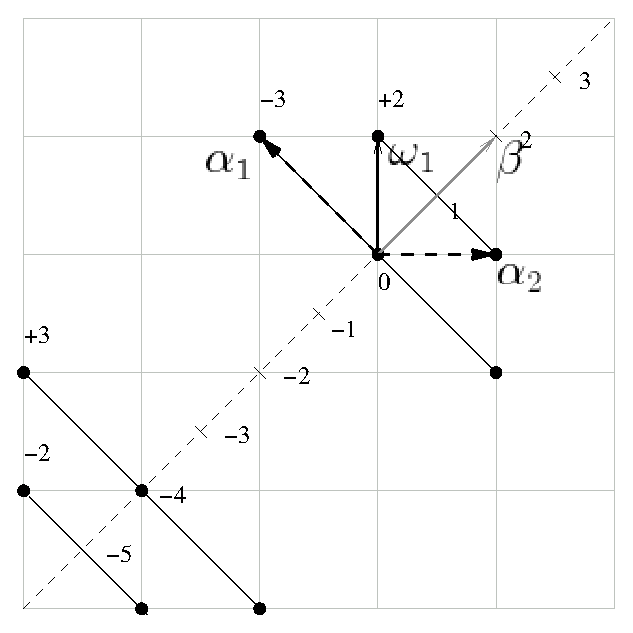
\includegraphics[width=60mm]{figures/figure2}
      \caption{Orthogonal subalgebra $\mathfrak{b}$ and $\mathfrak{b}$-module dimensions}
    \end{multicols}
  \end{figure}
\end{frame}
\begin{frame}
  \frametitle{Surprises}
  \begin{figure}[t]
    \vspace*{-0.5cm}
    \begin{multicols}{2}
      \hfill
        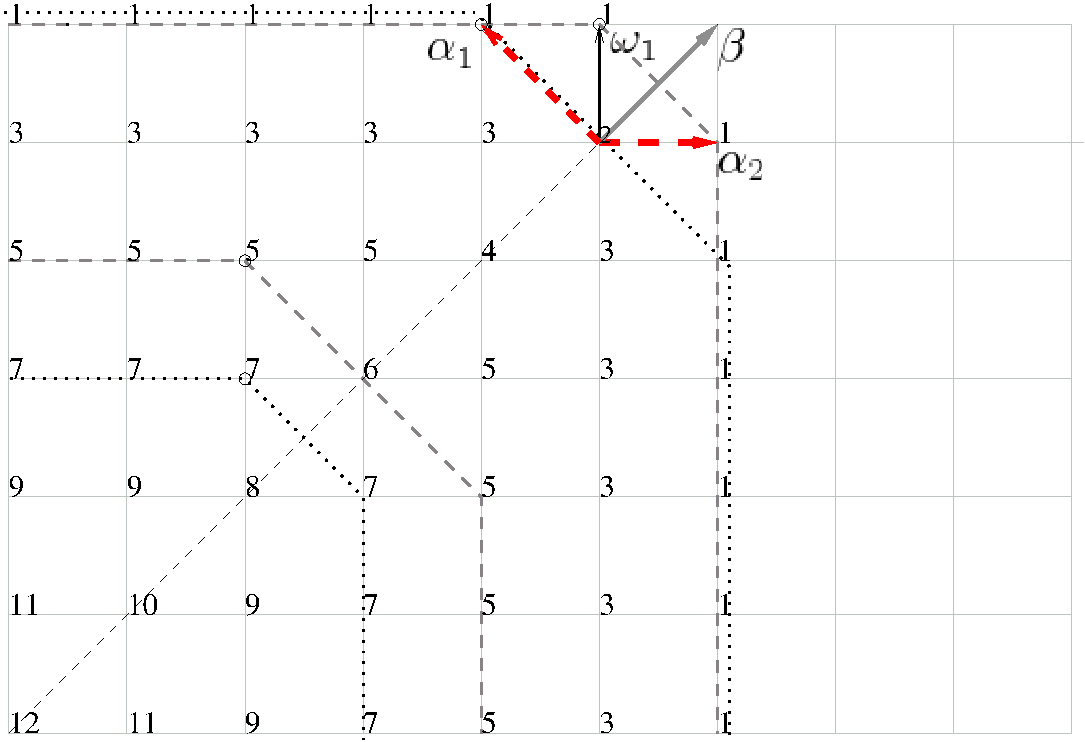
\includegraphics[width=60mm]{figures/B2_Gen_Verma_Decomp}
      \hfill
      \caption{Embedding $A_{1}\oplus u(1) \subset B_{2}$ and generalized Verma modules.
        Dashed -- positive $\epsilon(u)$, dotted --  negative.}
      \hfill
      \includegraphics[width=60mm]{figures/B2_A1_A2}
      \caption{Embedding $A_{1}\oplus u(1) \subset B_{2}$ and (deformed) $A_{2}$-modules}
    \end{multicols}
  \end{figure}
\end{frame}
\begin{frame}
  \begin{figure}[t]
    \vspace*{-0.5cm}
    \begin{multicols}{2}
      \hfill
      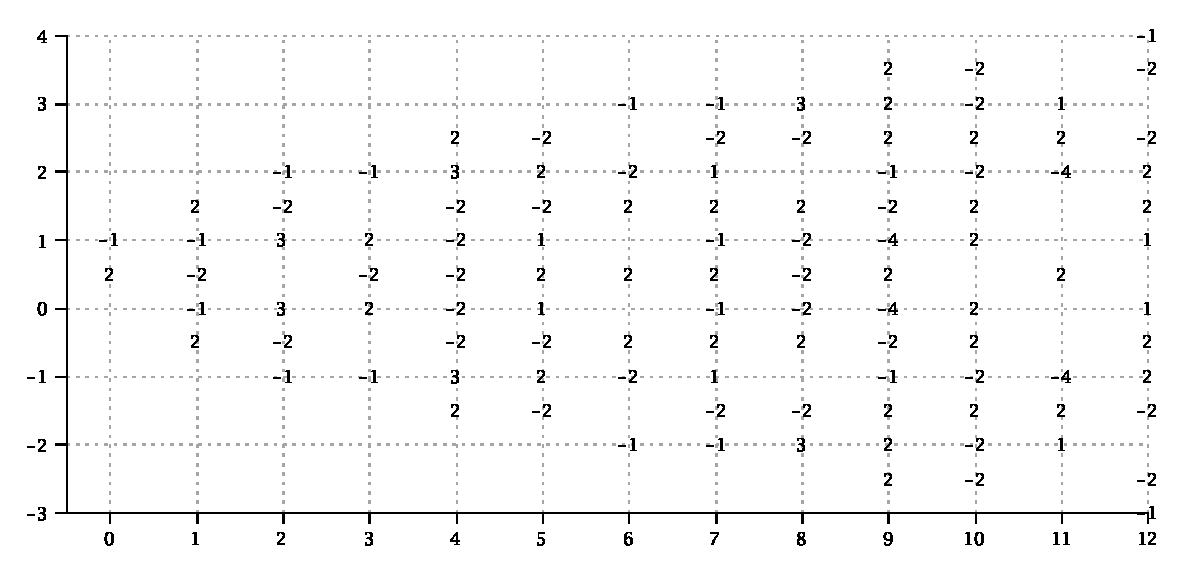
\includegraphics[width=60mm]{figures/figure10}
      \hfill
      \caption{$\Gamma_{\hat A_1\subset \hat B_2}$}
      \hfill
      \includegraphics[width=60mm]{figures/figure12}
      \caption{ $\pi_{\hat A_{1}}\left( \Psi ^{\omega_1  }_{\hat B_{2}}\right)$}
    \end{multicols}
  \end{figure}
  \begin{figure}[b]
    \vspace*{-1.3cm}
    \centering
      \includegraphics[width=100mm]{figures/figure13}
    \caption{(Signed) Branching coefficients for $\hat A_1\subset \hat B_2$}
    \label{fig:2}
  \end{figure}
\end{frame}

\begin{frame}
  \frametitle{Affine case}
  \begin{itemize}
  \item Infinite number of generalized Verma modules -- in each grade containing weights of singular element $\Psi$
  \item Not so simple relation with multiplicities of another algebra.\\
     $\Gamma_{\afh\subset \gfh}\nleftrightarrow \prod_{\alpha\in \Delta^{+}}\left(1-e^{-\alpha}\right)^{\mathrm{mult}(\alpha)}$ due to the difference in imaginary roots. E.g. $\widehat{A_{1}\oplus u(1)}\subset \hat B_{2}$:
    \begin{multline*}
      \frac{\cancel{\prod_{n>0} (1-e^{-n\delta})^{2}} \cancel{\prod_{n\geq 0}(1-e^{-\alpha_{1}-n\delta})}\dots }{\cancel{\prod_{n>0} (1-e^{-n\delta})^{2}} \cancel{\prod_{n\geq 0}(1-e^{-\alpha_{1}-n\delta})}\dots}\\ 
      \prod_{n\geq 0}(1-e^{-\alpha_{2}-n\delta}) 
        \prod_{n\geq 0}(1-e^{-\alpha_{1}-\alpha_{2}-n\delta}) \prod_{n\geq 0}(1-e^{-\alpha_{1}-2\alpha_{2}-n\delta}) \dots\\
        \nleftrightarrow \prod_{n>0} (1-e^{-n\delta})^{2} \prod_{n\geq 0}(1-e^{-\alpha_{1}-n\delta}) 
        \prod_{n\geq 0}(1-e^{-\alpha_{2}-n\delta})\\ \prod_{n\geq 0}(1-e^{-\alpha_{1}-\alpha_{2}-n\delta}) \dots
    \end{multline*}
  \end{itemize}
\end{frame}

\section{Conclusion}
\begin{frame}
  \frametitle{Conclusion}
  \begin{itemize}
  \item Recurrent relation for branching coefficients works as in finite-dimensional case
  \item It can be used for computations 
  \item We can relate recurrent relations for branching coefficients of one pair algebra-subalgebra with recurrent relation of another pair, but we can not interpret singular weights as highest weights of Verma modules.\\
    \begin{multicols}{2}
      E.g.: $\widehat{A_{1}\oplus u(1)}\subset \hat B_{2} \longleftrightarrow \widehat{u(1)\oplus u(1)}\subset \hat A_{2}$, \\
      or $\hat A_{2} \subset \hat G_{2} \longleftrightarrow \widehat{u(1)\oplus u(1)}\subset \hat A_{2}$      \\
    \includegraphics[width=40mm]{figures/G2-color}
    \end{multicols}
  \end{itemize}
\end{frame}
\begin{frame}
  \frametitle{Thank you for your attention!}
\end{frame}
\end{document}
